\graphicspath{{chapters/15/images/}}
\chapter{Protein motions}

\section{Elastic network models (ENM)}
In elastic network models ENM the structure of the protein is considered, with no attention to the kind of interactions.
The focus is on the topology: the protein is seen as a network of springs that connect beads.

\begin{figure}[H]
	\centering
	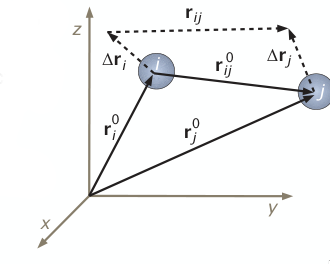
\includegraphics[scale = 0.5]{enm-theory}
	\caption{Elastic network models}
	\label{fig:enm-theory}
\end{figure}

Now considering the Gaussian network model, a kind of elastic network model.
Let $i$ and $j$ be two amino-acids as seen in \ref{fig:enm-theory}.
Usually the analysis is limited to centroids of residues: its $\alpha$-carbon atom.
A protein is represented by a configuration vector with the position of all its $\alpha$-carbon atoms: $\vec{r} = [\vec{r}_1, \vec{r}_2, \dots, \vec{r}_N]$.
It can be assumed that the structure obtained from the protein data bank is equilibrated.
Now computing the deviation of each $\alpha$-carbon atom from the equilibrium position (PDB structure):

$$\Delta\vec{r}_i = \vec{r}_i-\vec{r}_i^0$$

Instantaneous changes in the positions of all residues can be recorded in a vector with $3N$ components:

$$\Delta\vec{r} = [\Delta\vec{r}_1, \Delta\vec{r}_2, \dots, \Delta\vec{r}_N]$$


The equilibrium separation between two beads $i$ and $j$: $\vec{r}_{ij}^0 = \vec{r}_j^0-\vec{r}_i^0$.
The instantaneous separation between two beads $i$ and $j$: $\vec{r}_{ij} = \vec{r}_{ij}^0+\Delta\vec{r}_{ij}$, $\Delta\vec{r}_{ij} = \Delta\vec{r}_i-\Delta\vec{r}_i$.

	\subsection{Gaussian network model (GNM)}
	In Gaussian network model a potential energy is built up and it is assumed that each couple interact through an harmonic potential.
	So the potential energy for each couple:

	$$U_{ij} = \gamma_{ij}(\Delta\vec{r}_j-\Delta\vec{r}_i)\cdot(\Delta\vec{r}_j-\Delta\vec{r}_i) = \gamma_{ij}\Delta\vec{r}_{ij}^2$$

	Where the constant $\gamma$ depends on the couple of amino acid that are interacting.
	Now total elastic energy can be written as:

	$$U_{GNM} = \frac{1}{2}\sum\limits_i\sum\limits_j\gamma_{ij}\Delta\vec{r}^2_{ij} = \frac{\gamma}{2}\sum\limits_i\sum\limits_j\Delta\vec{r}_{ij}^2$$

	Another assumption, which is less problematic than the first one, does not affect the result.
	This assumption states that all amino acids that are interacting they interacting with the same constant $\gamma$ for all the couples there are.
	All the spring between the beads are the same.
	An interaction between two $\alpha$-carbon happens when they are closer than a cut-off radius usually set at $r_c = \si{\angstrom}$.
	Now Kirchhoff adjacency matrix $\Gamma$ is built, such that there is a $1$ (the sign is a convention) whenever there is an interaction or $0$ otherwise.
	This matrix will be symmetrical and the negative of the sum of rows or column and will be put on the diagonal.
	So in the diagonal there is the number of neighbours for each bead.

	\begin{figure}[H]
		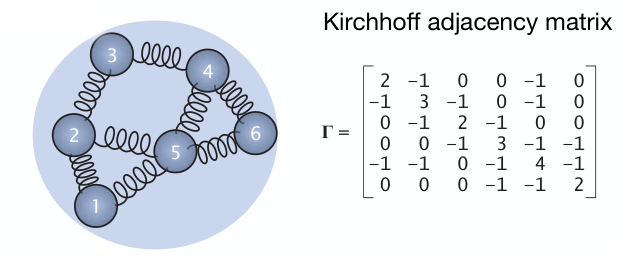
\includegraphics[width=\textwidth]{kirchoff-adjacency-matrix}
		\caption{Kirchhoff adjacency matrix}
		\label{fig:kirchhoff-adjacency}
	\end{figure}

	So the total elastic energy:

	$$U_{GNM} = \frac{\gamma}{2}\Delta\vec{r}(t)^T\Gamma\Delta\vec{r}(t)$$

		\subsubsection{Correlated motions}
		The average of displacement for each amino-acid and the correlated motion, so whether the displacement of an amino-acids correlates with the movement of another.
		To do so:

		$$\langle\Delta\vec{r}_i\cdot\Delta\vec{r}_j\rangle = \frac{1}{Q}\int\Delta\vec{r}_i\cdot\Delta\vec{r}_je^{-\frac{U}{kT}}d^N\Delta\vec{r}$$

		Since $U$ can be written as a matrix product the integral is a generalized Gaussian integral:

		$$\langle\Delta\vec{r}_i\cdot\Delta\vec{r}_j\rangle = \frac{3kT}{\gamma}[\Gamma^{-1}]_{ij}$$

		So that it can be exactly computed.
		Where $\Gamma^{-1}$ is a pseudoinverse matrix as the Kirchhoff matrix has zero determinant and cannot be inverted.
		To build the pseudoinverse matrix consider the eigenvalue decomposition: $\Gamma = U\Lambda U^T$:

		$$U = [\vec{u}_1, \dots, \vec{u}_{N_1}] = \begin{bmatrix} u_{1,1} & \cdots & u_{N-1,1}\\\vdots & \cdots & \vdots\\ u_{1, N} & \cdots & u_{N-1, N}\end{bmatrix}\qquad\Lambda = \begin{bmatrix} \lambda_1 & 0 & 0 & \cdots & 0\\ 0 & \lambda_2 & 0 &\cdots & 0\\0 & 0& \lambda_3 & \cdots & 0\\\vdots & \vdots & \vdots & \vdots &\vdots\\ 0 & 0 & 0 & \cdots & \lambda_{N-1}\end{bmatrix}$$

		Where $U$ is the matrix of eigenvectors and $\lambda_0$ is discarded.
		The pseudoinverse matrix is obtained by this matrix multiplication discarding $\lambda_0$ in $\Lambda$.

		\subsubsection{Gaussian network model and B-factors}
		Considering the average fluctuation and the correlation of amino-acids, if $i=j$ is the average fluctuation for each fluctuation, which can be obtained from the diagonal elements of the pseudoinverse matrix is:

		$$\langle\Delta\vec{r}_i\cdot\Delta\vec{r}_i\rangle = \frac{3kT}{\gamma}[U\Lambda^{-1}U^{T}]_{ii} = \frac{3kT}{\gamma}\sum\limits_{k}[\lambda_k^{-1}\vec{u}_k\vec{u}_k^T]_{ii} = \sum\limits_{k}[\Delta r_i^2]_k$$

		The root-mean squared deviation can be represented as a sum of fluctuation for each of the modes or eigenvectors.
		Considering the Debye-Waller factors:

		$$B_i = \frac{8\pi^2}{3}\langle\Delta r_i^2\rangle$$

		Which are found in the PDB file and the factor $\gamma$ can be obtained by comparison of a result of the Gaussian network model so that the data look similar to the Debye-Waller factors.
		In figure \ref{fig:gnn-b-factors} the Debye-Waller are the continuous line while the dotted line is the average fluctuation computed from the Gaussian network model.
		Pay attention to proximity effects that arise from the crystal structure.

		\begin{figure}[H]
			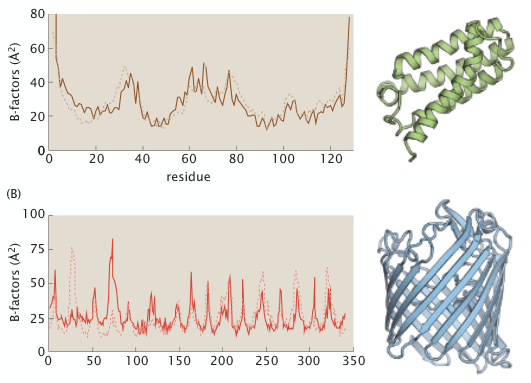
\includegraphics[width=\textwidth]{gnm-b-factors}
			\caption{GNM and B-factors}
			\label{fig:gnn-b-factors}
		\end{figure}

		\subsubsection{Biological relevance}
		Focussing on the slow of figure \ref{fig:biological-relevance} the contribution of each mode to the root mean squared deviation scales with the $-1$ power with respect to the eigenvalues: the smaller eigenvalue contribute more to the fluctuation and are the one more spread over the region of the protein.
		Looking at the fast mode with high eigenvalue are usually concentrated and characterized with spikes and are localized on amino-acids that corresponds to hydrophobic pocket of the protein and are fundamental for their structure.
		Inserting a mutation on one of the amino-acids could make the structure unstable.

		\begin{figure}[H]
			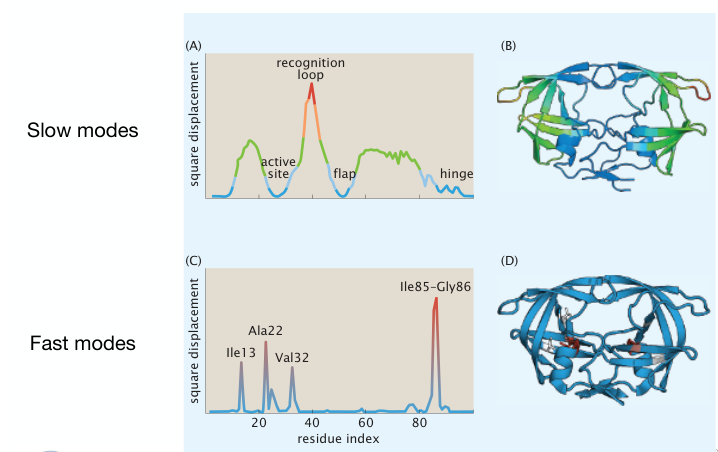
\includegraphics[width=\textwidth]{biological-relevance}
			\caption{Biological relevance}
			\label{fig:biological-relevance}
		\end{figure}

		\subsubsection{Normal mode analysis}
		Assuming that the approximation of the GNM is too crude and considering the fact that there are $3N-6$ degree of freedom.
		To be more rigorous the atomistic force field should be used and the potential function should be expanded through a Taylor expansion around an equilibrium position:

		$$U = U_0 + \sum\limits_i\frac{\partial U}{\partial q_i}\biggr\rvert_{q^0}(q_i-q_i^0) + \frac{1}{2}\sum\limits_i\sum\limits_j\frac{\partial^2 U}{\partial q_i\partial q_j}\biggr\rvert_{q^0}(q_i-q_i^0)(q_j-q_j^0) + \cdots$$

		If $q^0$ represent the equilibrium the sum of the forces and in turn the first order term will be equal to $0$, so at equilibrium:

		$$U = \frac{1}{2}\Delta\vec{q}^TH\Delta\vec{q} = \frac{1}{2}\sum\limits_i\sum\limits_j H_{ij}(q_i-q_i^0)(q_j-q_j^0)$$

		Where $H$ is the Hessian matrix:

		$$H_{ij} = \frac{\partial^2 U}{\partial q_i\partial q_j}\biggr\rvert_{q^0}$$

		A matrix that can be computed analytically or numerically.
		This process is expensive because numerical derivatives have to be taken, but it is cheaper with respect to a molecular dynamics simulation.
		Now a covariance matrix can be computed:

		$$C = \langle\Delta\vec{q}\Delta\vec{q}^T\rangle = \frac{1}{Q}\int\Delta\vec{q}\Delta\vec{q}^Te^{-\frac{\Delta\vec{q}^TH\Delta\vec{q}}{2kT}}d^N\Delta\vec{q} = kTH^{-1}$$

		Where $H^{-1}$ is a pseudoinvers as the Hessian matrix will have $6$ $0$-eigenvalues because the degrees of freedom are $3N-6$ because overall translations and rotations are excluded.

	\subsection{Anisotropic network model (ANM)}
	In the anisotropic network model a normal mode analysis is performed, while assuming that each pair of interacting amino-acids have the same constant $\gamma$ and there is an harmonic potential between them:

	$$U_{ANM} = \frac{1}{2}\sum\limits_{ij}\gamma(r_{ij}-r_{ij}^0)^2\Rightarrow\frac{\partial^2 U}{\partial x_i\partial y)i} = -\gamma\frac{(x_i-x_i)(y_i-y_j)}{t_{ij}^2}$$

	So now the Hessian matrix can be computed easily:

	$$H_{ij} = \frac{\gamma}{r_{ij}^2}\begin{bmatrix}x_{ij}^2 & x_{ij}y_{ij} & x_{ij}z_{ij}\\x_{ij}y_{ij} & y_{ij}^2 & y_{ij}z_{ij}\\ x_{ij}z_{ij} & y_{ij}z_{ij} & z_{ij}^2\end{bmatrix}$$

	This matrix will be a $N\times N$ matrix with each amino acid and all the elements are $3\times 3$ matrices.
	Now the eigenvalue decomposition $H=U\Lambda U^T$ can be performed and the $0$-eigenvalue will be discarded.

	$$\Lambda = \begin{bmatrix}\lambda_1 & 0 & 0 & \cdots & 0\\ 0 & \lambda_2 & 0 & \cdots & 0\\ 0 & 0 & \lambda_3 & \cdots & 0\\\vdots & \vdots & \vdots & \vdots & \vdots\\ 0 & 0 & 0 & \cdots & \lambda_{3N-6}\end{bmatrix}$$

		\subsubsection{Correlated motions}
		Computing now the correlation between amino-acids and focussing on the specific motion of each mode represented by an eigenvector.

		$$\langle\Delta\vec{r}_i\cdot\Delta\vec{r}_j\rangle = \frac{3kT}{\gamma}[U\Lambda^{-1}U^T]_{ij} = \frac{3kT}{\gamma}\sum\limits_{k}\lambda_k^{-1}[\vec{u}_k\vec{u}_k^T]_{ij}$$

		The displacement of a protein can be computed from the modes.
		The direction of each mode is considered.
		This model does not treat all direction as the same.

		\begin{figure}[H]
			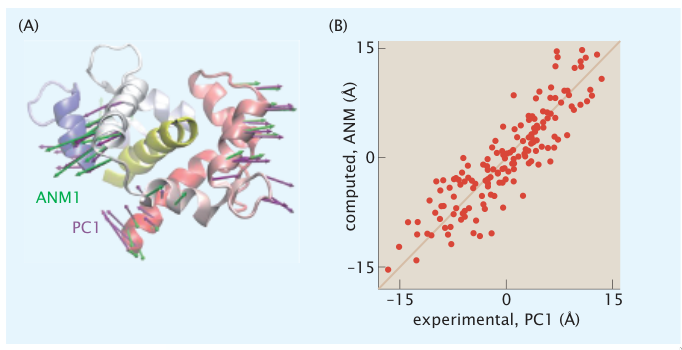
\includegraphics[width=\textwidth]{asm-correlated-motion}
			\caption{Correlated motions}
			\label{fig:as-correlated-motion}
		\end{figure}

		There are other instructive quantities that tells something more on the motion of the protein.
		For example the correlation cosine: projecting an eigenvector to the displacement between state $A$ and $B$ of the protein.
		The objective is to determine whether the transition was determined by the mode in consideration.
		The correlation cosine is computed as:

		$$I_k = \frac{\Delta\vec{q}_{AB}\cdot\vec{u}_k}{|\Delta\vec{q}_{AB}|}\qquad \Delta\vec{q}_{AB} = \vec{q}^B-\vec{q}^A$$

		The cumulative overlap is the number of mode that contribute to a motion:

		$$C_0 = \sqrt{\sum\limits_k I_k^2}$$

		Another quantity is the degree of collectivity, which will also be used in PCA.
		It is a factor that looks like a Shannon-entropy and it is defined as:

		$$\kappa_k = N^{-1}e^{-\sum\limits_{i=1}^N\alpha(\Delta r_i)^2\rvert_k\log(\alpha\Delta r_i)^2\rvert_k}$$

		Where $\alpha$ is normalized.

		$$\sum\limits_{i=1}^N\alpha(\Delta r_1)^2\rvert_k = 1$$

		When the degree of collectivity is close to $1$ there is a collective mode, so a mode that involves a large number of residues, while when it is close to $0$ the motion is localized on some portion of the protein.

\section{Essential dynamics}
Essential dynamics is based on principal component analysis: once a trajectory is obtained from a molecular dynamics simulation, the objective is to reduce the number of degrees of freedom to just those that are relevant to describe the motion of the system.
Not all of the degrees of freedom and a proper transformation of variable can be found so that the relevant of degrees of freedom are found.
They can be computed starting from the result of a molecular dynamics simulation.

\begin{enumerate}
	\item Obtain trajectories from molecular dynamics simulations, better if equilibrated.
		Equilibration is not mandatory as the new set of coordinates can be not equilibrated.
		There might be more than one trajectory that can be compared.
	\item Remove overall translations and rotations by aligning each frame to a reference structure.
		The reference frame can be the starting frame.
	\item Choose the set of atoms for the analysis like $\alpha$-carbons.
		In principle this analysis can be performed on all the atoms, but this is pointless.
		It is better to select on a subset of atoms, focussing on $\alpha$-carbons or on one sub-region of the protein.
	\item Obtain the covariance matrix:

		$$C_{ij} = \overline{(x_i(t) - \overline{x_i(t)})(x_j(t)-\overline{x_j(t)})}$$

		The covariance matrix is an average in time.
	\item If the fluctuations display some non-homogeneous behaviour, for example when there are loops that fluctuates a lot, it is better to employ the correlation matrix:

		$$R_{ij} = \frac{\overline{(x_i(t)-\overline{x_i(t)})}\overline{(x_j(t)-\overline{x_j(t)})}}{\sigma_{x_i}\sigma_{x_j}}$$

		Which is the covariance matrix normalized by the standard deviation.
	\item Diagonalize $C$ or $R$ employing eigenvalue decomposition EVD as in elastic network models.
	\item Examine the eigenvalue scree plot to determine the number of eigenvectors to include in the reduced vector space that describes the most relevant features.
		An example can be seen in figure \ref{fig:eigenvalue-scree-plot}.
		It can be seen how after a number of eigenvalues the other components have small eigenvalues.
		This behaviour is typical for a protein simulation, if the interaction describe a network.

	\begin{figure}[H]
	\centering
		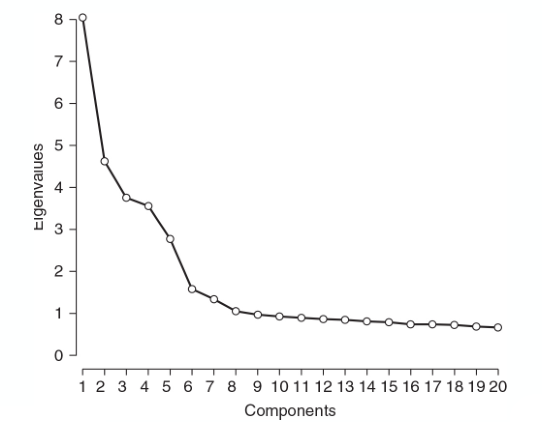
\includegraphics[scale = 0.5]{eigenvalue-scree-plot}
		\caption{Eigenvalue scree plot}
		\label{fig:eigenvalue-scree-plot}
	\end{figure}

\item Select the top set of eigenvectors to form the principal components (PCs) (usually between $2$ an $20$).
\item Examine the eigenvector collectivity for each mode defined as in the ANM: top modes tend to be more collective than lower modes, indicating that many residues are participating in collective motions.

	\begin{figure}[H]
	\centering
		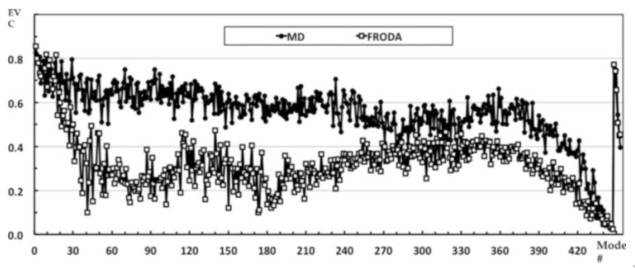
\includegraphics[scale = 0.4]{eigenvalue-collectivity}
		\caption{Eigenvalue collectivity}
		\label{fig:eigenvalue-collectivity}
	\end{figure}

\item Construct the weighted RMSD modes $\langle\Delta\vec{r}_i^2\rangle_k = \lambda_k[\vec{u}_k\vec{u}_k^T]_{ij}$.
	Visualize which residues contribute most to the fluctuation of each PCA mode.
	Comparing against the overall RMSD and looking where the most important contribution on the movement as in \ref{fig:weighted-rmsd}

	\begin{figure}[H]
	\centering
		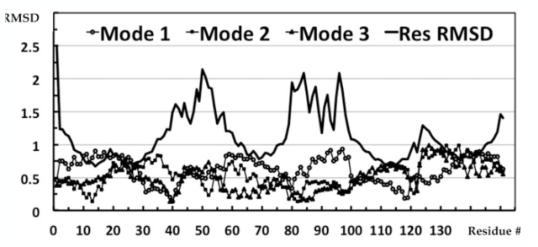
\includegraphics[scale = 0.4]{weighted-rmsd}
		\caption{Weighted RMSD modes}
		\label{fig:weighted-rmsd}
	\end{figure}

\item Construct the displacement vectors $\vec{d}_i(t) = \vec{r}_i(t)-\overline{\vec{r}_i}$ for each snapshot and construct the PCs projecting the displacement vectors onto the eigenvectors obtained:

	$$PC_k(t) = \sum\limits_{i=1}^N\vec{d}_i(t)\cdot\vec{u}_i^k\qquad\text{ with }k=1, \dots, 3N-6$$

	Each snapshot now is described by a single point with $3N-6$ numbers.
	Looking at these point in the multi-dimensional space and plotting them onto the first two principal component as in figure \ref{fig:scatter-plot-pcs-modes}.

	\begin{figure}[H]
	\centering
		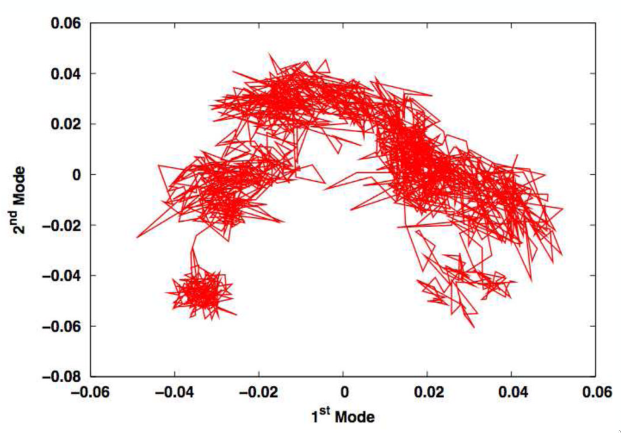
\includegraphics[scale = 0.4]{scatter-plot-pcs-modes}
		\caption{Scatter plot of first and second mode for PCs}
		\label{fig:scatter-plot-pcs-modes}
	\end{figure}

	The snapshots can be coloured according to time so to see the movement in the space as in figure \ref{fig:scatter-plot-pcs}

	\begin{figure}[H]
		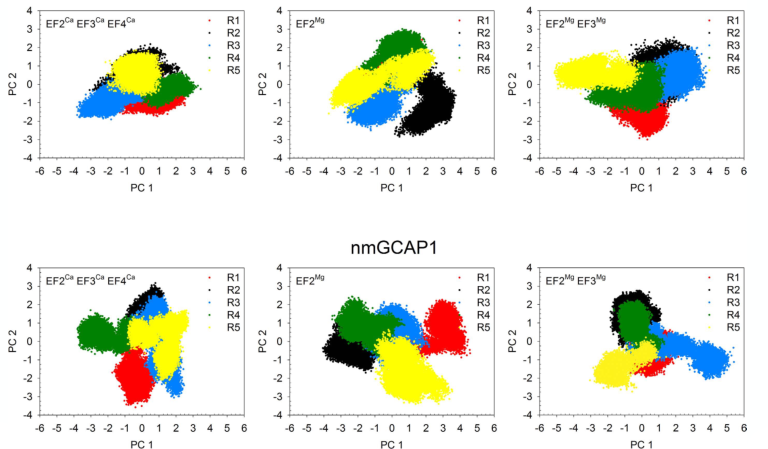
\includegraphics[width=\textwidth]{scatter-plot-pcs}
		\caption{Scatter plot of PCs, different replicas, the color indicates time of simulation.}
		\label{fig:scatter-plot-pcs}
	\end{figure}

\item Examine the cosine content for each mode $k$, defined as the superposition with the cosine obtained from a simple diffusion in a high dimensional harmonic potential:

	$$c_k = \frac{2}{T_{sim}}\left(\int_0^{T_{sim}}\cos\left(\pi\frac{k_BT}{\lambda_k}t\right)PC_k(t)dt\right)^2\left(\int_0^{T_{sim}}PC_k^2(t)dt\right)^{-1}$$

	The cosine content compares the principal component, which are a function of time, representing a time-series to the trajectory with the cosine that represents the diffusion of the system in a high-dimensional harmonic potential.
	If it is equal to $1$ one single basin is being explored, so the smaller the better, so that the system explores more basins and has equilibrated.
	An example can be seen in \ref{fig:cosine-content}.
	It can be seen how the cosine content decrees along the time of the simulation.
	The error bars can be obtained performing several simulation or dividing a simulation into pieces.
	This is another way to measure whether the system has equilibrated or not.

	\begin{figure}[H]
	\centering
		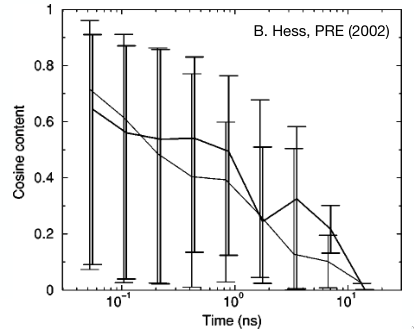
\includegraphics[scale = 0.6]{cosine-content}
		\caption{Cosine content for the modes}
		\label{fig:cosine-content}
	\end{figure}

\item Examine the similarity between trajectories or between portions of the same trajectory by examining the Covariance overlap:

	$$\Omega_{A, B} = 1 - \left[\frac{\sum\limits_{k=1}^{3N-6}(\lambda_k^A+\lambda_k^B)-2\sum\limits_{k=1}^{3N-6}\sum\limits_{j=1}^{3N-6}\sqrt{\lambda_k^A\lambda_j^B}(\vec{u}_k^A\cdot\vec{u}_j^B)^2}{\sum\limits_{k=1}^{3N-6}(\lambda_k^A+\lambda_k^B)}\right]^{\frac{1}{2}}$$

	$\Omega_{A, B} = 1$ if and only if the two covariance matrices are identical, while it is zero when the sampled subspaces are completely orthogonal.
\end{enumerate}
